\documentclass[conference]{IEEEtran}

% ---------- Packages ----------
\usepackage{graphicx}
\usepackage{amsmath,amssymb}
\usepackage{siunitx}
\usepackage{booktabs}
\usepackage{xcolor}
\usepackage{hyperref}
\usepackage{placeins} % \FloatBarrier
\usepackage{tikz}
\usetikzlibrary{positioning,arrows.meta,shapes,fit}

% TikZ styles (共通)
\tikzset{
  box/.style   ={draw, rounded corners=2pt, inner sep=4pt, align=center},
  step/.style  ={draw, rounded corners=2pt, inner sep=4pt, align=center},
  small/.style ={font=\small},
  tiny/.style  ={font=\footnotesize},
  arrow/.style ={->, >=Stealth}
}

% ---------- Title ----------
\title{AITL on Space: A Robust Three-Layer Architecture\\
with a Tri-NVM Hierarchy (SRAM / MRAM / FRAM)\\
for Long-Duration Spacecraft Autonomy}

\author{%
Shinichi Samizo\\
Independent Semiconductor Researcher\\
Former Engineer at Seiko Epson Corporation\\
Email: shin3t72@gmail.com \quad GitHub: \url{https://github.com/Samizo-AITL}
}

\begin{document}
\maketitle

% ----------------- Abstract (最優先で先に出す) -----------------
\begin{abstract}
We propose \emph{AITL on Space}, a three-layer control architecture (Robust Core, FSM Supervisor, AI Adaptor) implemented on a \SI{22}{nm} FDSOI SoC with a hardened tri-NVM hierarchy (SRAM/MRAM/FRAM). The system targets ultra-robust autonomy under radiation, thermal cycling, and long-term drift. This paper outlines the architecture, an 11D state-space plant model (8--20D extensible), an $H_\infty$ mixed-sensitivity design flow, and a verification pipeline from FPGA HIL to ASIC.
\end{abstract}

\section{Introduction}
Long-duration missions require high availability under TID/SEE and thermal cycles.
Conventional PID+Flash architectures face reliability limits.
We summarize related work and motivate AITL on Space.

\section{System Architecture}
AITL comprises: (i)~Robust Core (for $H_\infty$/MPC/SMC), (ii)~FSM Supervisor (Safe/Nominal/Recovery, FDI/FDI), and (iii)~AI Adaptor for long-term re-identification. A tri-NVM hierarchy---SRAM for execution, MRAM for logs/code (ECC+scrub, A/B slots), and FRAM for safe boot---ensures persistence.

% ---- Fig.1 (アーキテクチャ):Abstractの後に出るようにここで配置 ----
\begin{figure*}[!t]
  \centering
  \begin{tikzpicture}[node distance=8mm]
    % Left column: three layers
    \node[box, minimum width=3.4cm] (robust) {Robust Core\\ \small $H_\infty$/MPC/SMC};
    \node[box, below=6mm of robust, minimum width=3.4cm] (fsm) {FSM Supervisor\\ \small Safe/Nominal/Recovery\\ FDI/FDII};
    \node[box, below=6mm of fsm, minimum width=3.4cm] (ai) {AI Adaptor\\ \small Re-ID / Drift Compensation};

    % Plant and blocks on the right
    \node[box, right=22mm of robust, minimum width=2.2cm] (att) {Attitude (6)};
    \node[box, right=10mm of att, minimum width=2.2cm] (bus) {Power Bus (2)};
    \node[box, right=10mm of bus, minimum width=2.2cm] (therm) {Thermal (3)};

    % Tri-NVM block under the chain
    \node[box, below=9mm of bus, minimum width=6.8cm, align=left] (nvm) {Tri-NVM Hierarchy\\
      \footnotesize SRAM: Exec\\
      \footnotesize MRAM: Code/Logs (ECC+Scrub, A/B)\\
      \footnotesize FRAM: Safe Boot \& FSM State};

    % Connections
    \draw[arrow] (robust.east) -| (att.west);
    \draw[arrow] (fsm.east) -| (att.west);
    \draw[arrow] (ai.east)  -| (att.west);
    \draw[arrow] (att) -- (bus);
    \draw[arrow] (bus) -- (therm);
    \draw[arrow] (nvm.north) -- ($(att.south)!0.5!(bus.south)$);

    % Decorative system boundary
    \node[draw, rounded corners=2pt, fit=(att)(bus)(therm), inner sep=8pt, label={[tiny]above:11D Plant}] {};
  \end{tikzpicture}
  \caption{AITL on Space architecture with Robust Core, Supervisor FSM, AI Adaptor, and the Tri-NVM hierarchy.}
  \label{fig:arch}
\end{figure*}

\section{Mathematical Model}
We use an 11D discrete-time plant that couples attitude (6), power bus (2), and thermal nodes (3):
\begin{align}
  x_{k+1} &= A x_k + B u_k + E w_k, \\
  y_k     &= C x_k + D u_k + v_k.
\end{align}
Extensions scale to 20D with translational axes and bias states.

% ---- Fig.2 (H∞ loop) ----
\begin{figure}[!t]
  \centering
  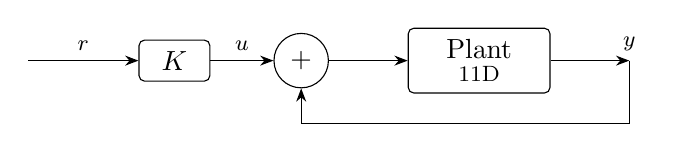
\begin{tikzpicture}
    % reference r and sum
    \node[box, minimum width=0.9cm] (K) {$K$};
    \node[coordinate, left=14mm of K] (r) {};
    \node[circle, draw, minimum size=10pt, right=8mm of K] (sum) {$\small +$};
    % plant (改行は \shortstack でLR mode回避)
    \node[box, right=10mm of sum, minimum width=1.8cm] (P) {\shortstack{Plant\\\footnotesize 11D}};
    % arrows
    \draw[arrow] (r) -- node[above, tiny]{$r$} (K.west);
    \draw[arrow] (K.east) -- node[above, tiny]{$u$} (sum.west);
    \draw[arrow] (sum.east) -- (P.west);
    \draw[arrow] (P.east) -- ++(10mm,0) node[above, tiny]{$y$} coordinate (yout);
    % feedback
    \draw[arrow] (yout) |- ++(0,-8mm) -| (sum.south);
  \end{tikzpicture}
  \caption{Closed-loop schematic used for $H_\infty$ synthesis on the 11D plant.}
  \label{fig:hinf}
\end{figure}

\section{$H_\infty$ Mixed-Sensitivity Design}
Weights $(W_1,W_2,W_3)$ shape sensitivity, effort, and complementary sensitivity.
EduController exports JSON plant/weights; AITL-H synthesizes output-feedback $K$ and fixed-point realization.

\section{Verification Pipeline}
FPGA HIL injects SEU bursts and sensor outages; metrics include safe-mode time ($<\SI{1}{s}$), recovery rate ($\ge \SI{99}{\%}$), and ECC statistics. Physical design proceeds to 22FDX tape-out; SystemDK FEM closes thermal/packaging.

% ---- Fig.3(検証フロー) ----
\begin{figure}[!t]
  \centering
  \begin{tikzpicture}[node distance=8mm]
    \node[step, fill=blue!8, minimum width=3.6cm] (json) {JSON Plant/Weights};
    \node[step, fill=green!10, below=of json, minimum width=3.6cm] (rtl) {RTL Synthesis};
    \node[step, fill=orange!12, below=of rtl, minimum width=3.6cm] (hil) {FPGA HIL};
    \node[step, fill=red!8, below=of hil, minimum width=3.6cm] (asic) {22FDX ASIC};

    \node[box, right=22mm of rtl, minimum width=4.2cm] (fem) {SystemDK FEM\\ \small Thermal / Radiation / Packaging};

    \draw[arrow] (json) -- (rtl);
    \draw[arrow] (rtl) -- (hil);
    \draw[arrow] (hil) -- (asic);
    \draw[arrow] (rtl) -- (fem);
  \end{tikzpicture}
  \caption{Verification pipeline from JSON design to RTL, FPGA HIL, and ASIC; FEM closes the loop with thermal and radiation scenarios.}
  \label{fig:flow}
\end{figure}

\section{Conclusion}
AITL on Space offers a practical path to resilient autonomy for deep-space missions.

% ----------------- References -----------------
\begin{thebibliography}{99}\footnotesize
\bibitem{Doyle}
G.~Doyle, \emph{Feedback Control Theory}.
\bibitem{Colinge}
J.-P.~Colinge, \emph{Silicon-on-Insulator Technology}.
\end{thebibliography}

% ----------------- Biography -----------------
\section*{Author Biography}
\noindent
Shinichi Samizo received the M.S. degree in Electrical and Electronic Engineering from Shinshu University, Japan. He worked at Seiko Epson Corporation as an engineer in semiconductor memory and mixed-signal device development, and contributed to inkjet MEMS actuators and PrecisionCore printhead technology. He is currently an independent semiconductor researcher focusing on process/device education, memory architecture, and AI system integration. Contact: \texttt{shin3t72@gmail.com}.
\end{document}
